\section{Array}
\subsection{Definitie}
\begin{frame}{Array: Definitie}
\begin{definition}[Array]
Een \term{\dsarray{}} is een gegevensstructuur die bestaat uit een opeenvolging van elementen. Elk element in een \dsarray{} heeft een unieke \term{index} en is toegankelijk in constante tijd (dit wordt ook wel \term{Random-Access} genoemd). Een \dsarray{} heeft een vaste \term{lengte} die bij de declaratie wordt toegekend. Eenmaal toegekend staat die lengte dus vast.
\end{definition}
%\begin{block}{Voorstelling}
Visueel zullen we een \dsarray{} in deze presentatie voorstellen als een opeenvolging van hokjes zoals hier:
\begin{figure}
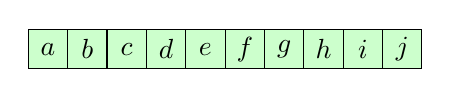
\begin{tikzpicture}
\filldraw[fill=green!20,draw=black] (0,0) rectangle (5,0.5);
\foreach \x in {1,2,...,9} {
  \draw (0.5*\x,0) -- ++(0,0.5);
}
\foreach \x/\t in {0/a,1/b,2/c,3/d,4/e,5/f,6/g,7/h,8/i,9/j} {
  \draw (0.5*\x+0.25,0.25) node {$\t$};
}
\end{tikzpicture}
\caption{Voorstelling van een \dsarray{}}
\end{figure}
%\end{block}
\end{frame}
\subsection{In Java}
\subsubsection{Declaratie}
\begin{frame}[fragile]{\dsarray{} in Java: declaratie}
In Java wordt een \dsarray{} aangemaakt door het type van de elementen te specificeren gevolgd door vierkante haken (\texttt{[]}). Tussen de vierkante haken wordt de lengte geplaatst:
\examplecode{Declaratie \dsarray{}}{arraydeclaration0}
\begin{hint}[Declaratie en toewijzing]
Indien men een array wil initialiseren waarbij de elementen ook al ingevuld worden, kan men gebruik maken van accolades:
\loadcode{arraydeclaration1}
\end{hint}
\end{frame}
\begin{frame}[fragile]{\dsarray{} in Java: declaratie: primitief versus klasse}
Java maakt een onderscheid tussen de declaratie van een array van \term{primitieve datatypes} (\dsint{}, \dsfloat{}, \dslong{},...) en \term{klasse-datatypes} (\dsobject{}, \dsstring{}):
\begin{enumerate}
 \item Bij primitieve datatypes wordt de \term{data} in de array opgeslagen.
 \begin{figure}[H]
 \centering
 \begin{tikzpicture}
 \tikzarray{10}{6,9,5,3,8,9,1,8,8,5}
 \end{tikzpicture}
 \end{figure}
 \item Bij klasse-datatypes worden \term{pointers} in de array opgeslagen.
 \begin{figure}[H]
 \centering
 \begin{tikzpicture}
 \tikzarrayptr{10}{paex}
 \begin{scope}[xshift=-2cm,yshift=1 cm]
 \strobj{e0}{Element 0}
 \end{scope}
 \begin{scope}[xshift=-1.5cm,yshift=-1 cm]
 \strobj{e1}{Element 1}
 \end{scope}
 \begin{scope}[xshift=0cm,yshift=1 cm]
 \strobj{e2}{Ander element}
 \end{scope}
 \begin{scope}[xshift=1cm,yshift=-1 cm]
 \strobj{e3}{Ander element 2}
 \end{scope}
 \draw[pointer] (paex1) -- (e0);
 \draw[pointer] (paex2) -- (e1);
 \draw[pointer] (paex4) -- (e2);
 \draw[pointer] (paex6) -- (e3);
 \draw[pointer] (paex7) -- (e3);
 \draw[pointer] (paex8) -- (e2);
 \draw[pointer] (paex10) -- (e3);
 \end{tikzpicture}
 \end{figure}
\end{enumerate}
\end{frame}
\subsubsection{Toegang tot elementen}
\begin{frame}[fragile]{\dsarray{} in Java: toegang tot elementen}
In Java kan men een element in een \dsarray{} opvragen door na de naam van de variabele tussen vierkante haken de index te vermelden. De index telt vanaf 0. Het eerste element staat dus op index 0. Men kan de waarde van een element in een array dan uitlezen en aanpassen.
\examplecode{Toegang tot elementen van een \dsarray{}}{arrayaccess0}
\end{frame}
\subsubsection{Lengte}
\begin{frame}[fragile]{\dsarray{} in Java: lengte}
In Java kan men de lengte van een \dsarray{} opvragen door het \texttt{length} argument op te roepen.
\examplecode{Lengte opvragen van een \dsarray{}}{arraylength0}
\end{frame}